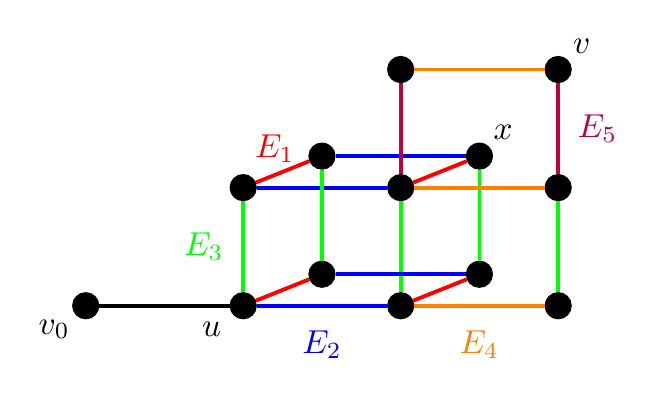
\begin{tikzpicture}

% NODES %%%%%%%%%%%%%%%%%%%%%%%%%%%%%%%%%%%%%%%%%%%%%%%%%%%%%%%%%%%%%%%%%%

\node[draw, circle, minimum height=0.2cm, minimum width=0.2cm, fill=black] (P01) at (-1,1) {};

\node[draw, circle, minimum height=0.2cm, minimum width=0.2cm, fill=black] (P11) at (1,1) {};
\node[draw, circle, minimum height=0.2cm, minimum width=0.2cm, fill=black] (P12) at (1,2.5) {};
\node[draw, circle, minimum height=0.2cm, minimum width=0.2cm, fill=black] (P13) at (3,1) {};
\node[draw, circle, minimum height=0.2cm, minimum width=0.2cm, fill=black] (P14) at (3,2.5) {};

\node[draw, circle, minimum height=0.2cm, minimum width=0.2cm, fill=black] (P21) at (2.0,1.4) {};
\node[draw, circle, minimum height=0.2cm, minimum width=0.2cm, fill=black] (P22) at (2.0,2.9) {};
\node[draw, circle, minimum height=0.2cm, minimum width=0.2cm, fill=black] (P23) at (4.0,1.4) {};
\node[draw, circle, minimum height=0.2cm, minimum width=0.2cm, fill=black] (P24) at (4.0,2.9) {};



\node[draw, circle, minimum height=0.2cm, minimum width=0.2cm, fill=black] (P31) at (3.0,4) {};
\node[draw, circle, minimum height=0.2cm, minimum width=0.2cm, fill=black] (P32) at (5.0,4) {};

\node[draw, circle, minimum height=0.2cm, minimum width=0.2cm, fill=black] (P41) at (5.0,1) {};
\node[draw, circle, minimum height=0.2cm, minimum width=0.2cm, fill=black] (P42) at (5.0,2.5) {};

%\node[draw, circle, minimum height=0.2cm, minimum width=0.2cm, fill=black] (P51) at (8.0,5.0) {};
%\node[draw, circle, minimum height=0.2cm, minimum width=0.2cm, fill=black] (P52) at (4.5,5.5) {};




% LINKS %%%%%%%%%%%%%%%%%%%%%%%%%%%%%%%%%%%%%%%%%%%%%%%%%%%%%%%%%%%%%%%%%%

\draw[line width = 1.4pt] (P01) -- (P11);

\draw[line width = 1.4pt, color = green] (P11) -- (P12);
\draw[line width = 1.4pt, color = blue] (P11) -- (P13);
\draw[line width = 1.4pt, color = red] (P11) -- (P21);
\draw[line width = 1.4pt, color = blue] (P12) -- (P14);
\draw[line width = 1.4pt, color = red] (P12) -- (P22);
\draw[line width = 1.4pt, color = red]  (P13) -- (P23);
\draw[line width = 1.4pt, color = green] (P13) -- (P14);
\draw[line width = 1.4pt, color = red]  (P14) -- (P24);
\draw[line width = 1.4pt, color = green] (P21) -- (P22);
\draw[line width = 1.4pt, color = blue] (P21) -- (P23);
\draw[line width = 1.4pt, color = green] (P23) -- (P24);
\draw[line width = 1.4pt, color = blue] (P22) -- (P24);

\draw[line width = 1.4pt, color = purple] (P14) -- (P31);
\draw[line width = 1.4pt, color = purple] (P42) -- (P32);
\draw[line width = 1.4pt, color = orange] (P13) -- (P41);
\draw[line width = 1.4pt, color = orange] (P14) -- (P42);
\draw[line width = 1.4pt, color = orange] (P31) -- (P32);
\draw[line width = 1.4pt, color = green] (P41) -- (P42);

%\draw[dashed] (P32) -- (P51);
%\draw[dashed] (P24) -- (P52);

% ETIQUETTES

\node[scale=1.2, color = red] at (1.4,3.0) {$E_1$};
\node[scale=1.2, color = blue] at (2.0,0.5) {$E_2$};
\node[scale=1.2, color = green] at (0.5,1.75) {$E_3$};
\node[scale=1.2, color = orange] at (4.0,0.5) {$E_4$};
\node[scale=1.2, color = purple] at (5.5,3.25) {$E_5$};

\node[scale = 1.2] at (-1.4,0.7) {$v_0$};
\node[scale = 1.2] at (0.6,0.7) {$u$};
%\node[scale = 1.2] at (2.6,2.2) {$u^+$};
\node[scale = 1.2] at (5.3,4.3) {$v$};
\node[scale = 1.2] at (4.3,3.2) {$x$};

\end{tikzpicture}
